\documentclass[10pt,a4paper]{article}
\usepackage[utf8]{inputenc}
\usepackage{amsmath}
\usepackage{amsfonts}
\usepackage{amssymb}
\usepackage{todonotes}
\usepackage{graphicx}

\begin{document}

\begin{titlepage}

\newcommand{\HRule}{\rule{\linewidth}{0.5mm}} % Defines a new command for the horizontal lines, change thickness here

\center % Center everything on the page
 
\textsc{\LARGE KU Leuven}\\[1.5cm] % Name of your university/college
\textsc{\Large 1 Ma Ingenieurswetenschappen: Computerwetenschappen}\\[0.5cm] % Major heading such as course name
\textsc{\large Bedrijfservaring: Computerwetenschappen}\\[0.5cm] % Minor heading such as course title


\HRule \\[0.4cm]
{ \huge \bfseries Stageverslag bedrijfservaring Alcatel-Lucent}\\[0.4cm]
\HRule \\[1.5cm]
 

\Large \emph{Author:}\\
Helena \textsc{Brekalo}\\[3cm]

{\large \today}\\[3cm] % Date

\vfill % Fill the rest of the page with whitespace

\end{titlepage}

Helena Brekalo\\
1e master Computerwetenschappen (Veilige software)\\
\medskip
\\
\textbf{Gegevens bedrijf:}\\
Alcatel-Lucent\\
Copernicuslaan 50\\
2018 Antwerpen\\
\medskip
\\
\textbf{Gegevens stagebegeleider:}\\
Bart Hemmeryckx-Deleersnijder\\
E-mail: bart.hemmeryckx-deleersnijder@alcatel-lucent.be\\
GSM-nummer: +32 472 95 00 65\\
Vast nummer binnen het bedrijf: +32 3 240 8525
\medskip
\\
\textbf{Stageperiode:}\\
1 juli - 7 augustus\\
7 september - 11 september
\clearpage

\begin{center}
\textbf{Abstract}

\end{center}
\tableofcontents
\clearpage

\section{Het bedrijf: Alcatel-Lucent}
Alcatel-Lucent is een Frans bedrijf met de hoofdzetel in Frankrijk en vestigingen in Amerika, Azi\"e, Europa (met dus onder andere een vestiging in Antwerpen), het Midden-Oosten \\todo{hoofdletters?} en Afrika. Alcatel kent een lange historie van overnames, met de meest recente overname die door Nokia, begin 2015.\\
De eerste funderingen van Alcatel werden gelegd in 1869, met de opstart van Gray and Barton in Cleveland, Ohio. Een tien jaar later worden ze overgenomen door American Bell, wat in 1925 leidt tot het ontstaan van Bell Telephone Laboratories. In deze "Bell Labs" worden verschillende grote ontwikkelingen verwezenlijkt, waaronder de eerste lange afstandstelevisietransmissie en de uitvinding van de batterij op zonne-energie. \todo{beter schrijven!} In 1984 worden ze overgenomen door C\^ables de Lyon en worden ze een Frans bedrijf. In 2006 mergen Alcatel en het Amerikaanse Lucent Technologies, waarop de naam verandert naar Alcatel-Lucent. In 2015 werd Alcatel-Lucent overgenomen door Nokia, wat effectief zal worden in april 2016. Door deze overname zal Nokia het tweede grootste bedrijf in wireless zijn, op Ericsson na. Op deze manier wordt de concurrentie met het Chinese Huawei vergroot op het gebied van draadloze communicatietechnologie.\\
Alcatel-Lucent heeft verschillende afdelingen, zijnde het \textit{core networking segment}, wat IP routing, transport en platforms omvat en het \textit{access segment}, wat wireless en fixed access omvat, alsook licensing en \textit{managed services}. In Antwerpen wordt er aan al deze segmenten gewerkt; zelf werd ik tewerkgesteld in de fixed access afdeling, namelijk Motive Network Analyzer-Copper (Motive NA-C). Zij staan ervoor in om het gebruik van het kopernetwerk te optimaliseren en fouten te detecteren en verhelpen.\\ \todo{nog tekst toevoegen?}


\section{Stage}
\subsection{Afdeling: Motive NA}
De stage ging door op de afdeling Motive Network Analyzer - Copper (NA-C) bij het team dat ook onder begeleiding staat van mijn stagebegeleider Bart Hemmeryckx-Deleersnijder. Motive NA-C heeft een team in Antwerpen, Chennai en Bangalor, waarbij de development voornamelijk in Antwerpen gebeurt en het testen in Chennai en Bangalor. Er zijn altijd ook enkele testers van Chennai en Bangalor in Antwerpen, om zo de communicatie tussen de teams te verbeteren en de samenwerking te vergemakkelijken.
\subsection{Werkmethoden}
\subsubsection{Scrum}
Het team van Bart werkt volgens de scrum-methode, zoals kort was aangehaald tijdens de hoorcollege's van Software-Ontwerp. Scrum is een voorbeeld van een agile werkmethode, waarbij men ervan uitgaat dat de vereisten voor het project kunnen en zullen veranderen gedurende het project. 
Bij het klassieke watervalmodel stelt men eerst de vereisten op, om deze vervolgens te implementeren, dit te evalueren en dan te onderhouden. Het probleem hierbij is dat de communicatie tussen de klant en het bedrijf 
niet optimaal verloopt, gezien de klant nog van gedachte kan veranderen over de requirements die hij wil. Als deze pas in de maintenance fase ontdekt en aangekaart worden, is het heel kostelijk om (grote) veranderingen opnieuw door te voeren.\\
Bij een agile werkmethode, waar scrum een onderdeel van is, gaat men er van uit dat de klant op voorhand niet perfect kan weten wat hij wil en dat hij dus de requirements zal aanpassen.\\
De term "scrum" is afkomstig vanuit rugby, waarbij de twee teams voorovergebogen tegen elkaar leunen, met de hoofden bij elkaar. De bal wordt dan in deze groep gegooid, waarop ze proberen om de bal als eerste in hun bezit te krijgen.\\
De gelijkenis met de software-ontwikkeling-scrum is dat het team heel nauw samenwerkt, inspeelt op veranderde omstandigheden en zo samen tot een doel komt. De samenwerking uit zich in dagelijkse stand-up meetings, waarbij iedereen vertelt wat hij/zij de dag ervoor heeft gedaan, welke problemen er eventueel zijn opgetreden en of er daar hulp bij nodig is en wat de planning voor de komende dag is. Op deze manier is iedereen op de hoogte van wie waarmee bezig is en kunnen problemen snel opgelost worden. Bij het NA-C team in Antwerpen maakt men hierbij ook gebruik van het agile dashboard van JIRA, waarbij gevisualiseerd wordt wie waarmee bezig is (zie Figuur \label{jira}). Indien iemand ergens problemen mee heeft, doet men aan pair-programming, waarbij men bij elkaar gaat zitten en samen nadenken over hoe het desbetreffende probleem opgelost kan worden en dit ook samen uit te werken.\\

\begin{figure}[ht!]
\centering
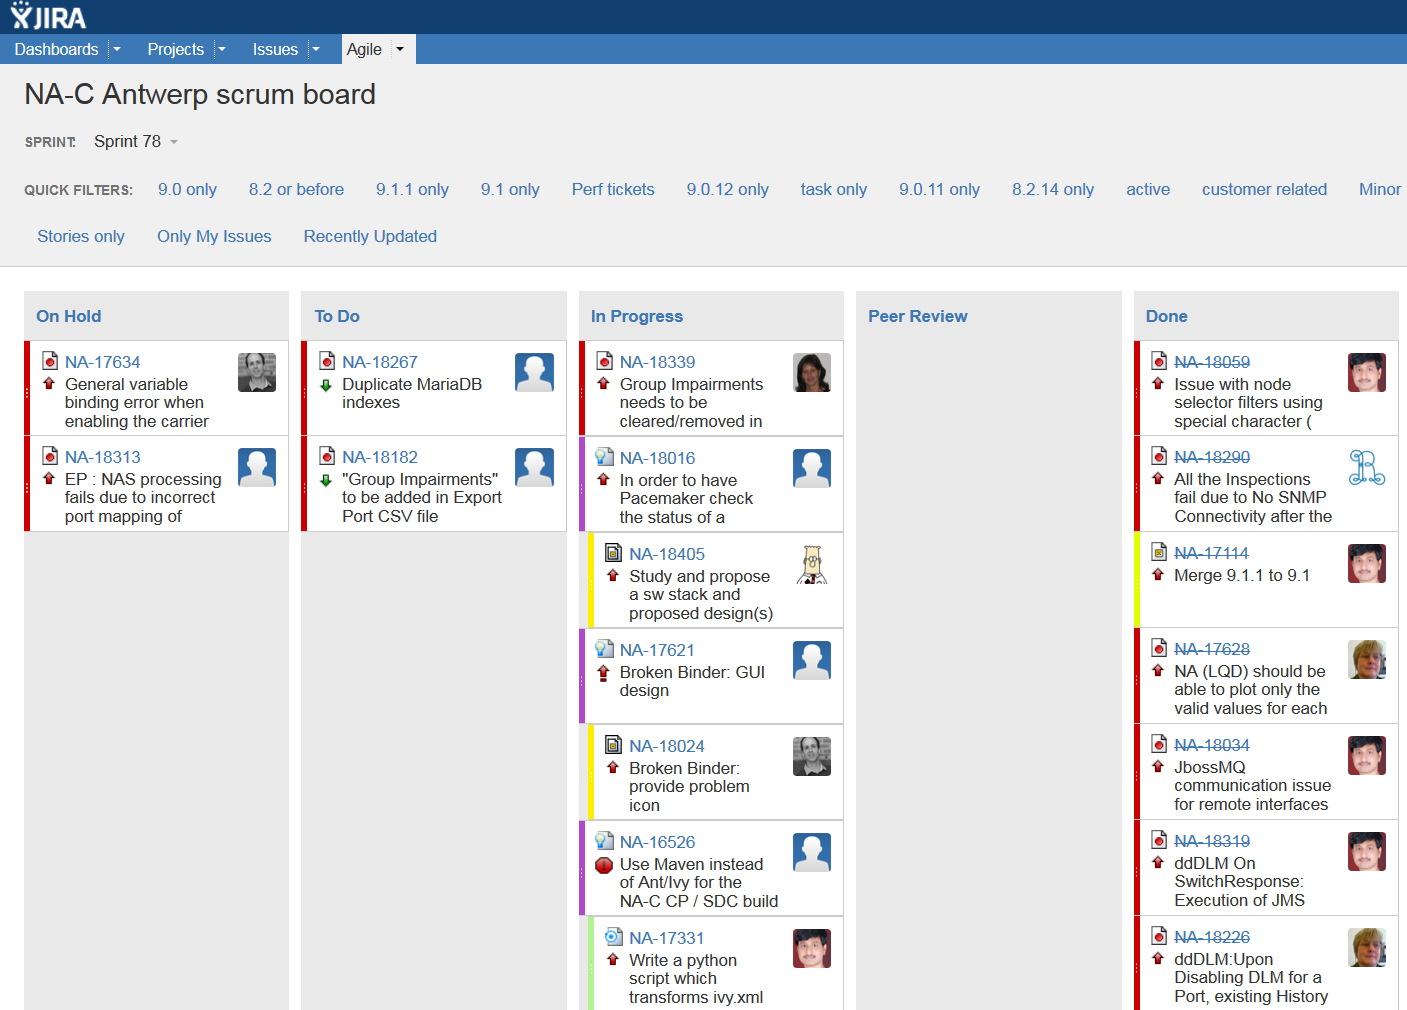
\includegraphics[width=90mm]{CaptureJira.png}
\caption{Het JIRA dashboard van het NA-C team in Antwerpen.} 
\label{jira}
\end{figure}

In het NA-C team heeft men sprints van twee weken, wat wil zeggen dat men elke twee weken een evaluatie doet van het werk dat in de afgelopen twee weken verzet is en waarbij eventueel demo's gegeven worden van wat er gerealiseerd is (sprint review). Samen met het einde van de sprint is er de sprint retrospective, waarbij men gaat oplijsten wat er goed en minder goed is gegaan, welke problemen er (binnen het team) waren en hoe deze opgelost kunnen worden. Aan het begin van een sprint is er dan de sprint planning, waarin er bekeken wordt wat er moet gebeuren met welke prioriteit en wie wat gaat doen (heel algemeen). Men maakt hierbij gebruik van user-stories, die een bepaalde taak omschrijven en de subtaken ervan. Het beschrijft wat de gebruiker nodig heeft bij het uitvoeren van zijn taak en bepalen zodus wat er moet ontwikkeld worden om de gebruiker hierbij te helpen. Het omschrijft het "wie", "wat" en "waarom" van deze vereisten op hoog niveau.
\subsubsection{Continuous integration}
Aangezien er regelmatig releases van software zijn, doet men aan continuous integration, wat inhoudt dat wanneer iemand klaar is met het schrijven van een stuk code en deze commit, alle builds en testen hierrond automatisch zullen runnen zodat fouten in een vroeg stadium kunnen gevonden en opgelost worden.\\
In Antwerpen maakt men gebruik van Jenkins\footnote{https://jenkins-ci.org/}, een open-source continuous integration systeem. Jenkins heeft een dashboard dat een overzicht toont van alle builds, maar je kan ook filteren op zelfgemaakte criteria, zodat je enkel de status van bepaalde builds ziet. Het overzicht toont een gekleurde bol om aan te geven of de laatste build geslaagt (groen/blauw) of gefaald is. Als er testen gefaald zijn, dan zal de bol geel kleuren.\\
Er is ook een weerbericht dat toont hoe stabiel de build is, waarbij slecht weer duidt op een instabiele build en goed weer op een stabiele build. Een screenshot van dit dashboard is te zien in Figuur \ref{jenkins}.

\begin{figure}[ht!]
\centering
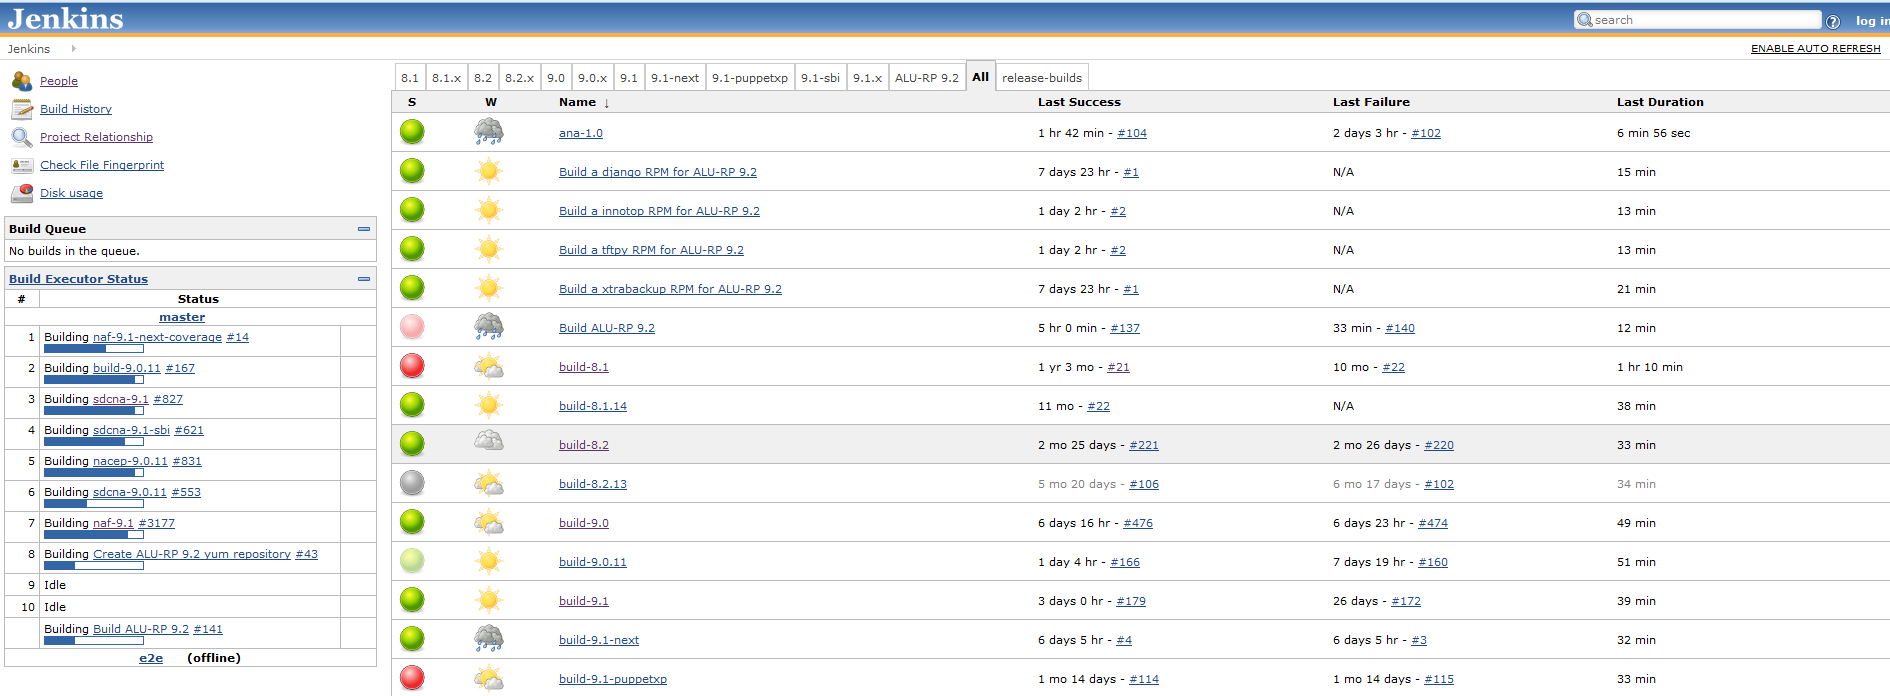
\includegraphics[width=90mm]{CaptureJenkins.png}
\caption{Het Jenkins dashboard, zoals origineel gebruikt op de afdeling NA-C in Antwerpen.} 
\label{jenkins}
\end{figure}

Het probleem met dit dashboard is dat het niet echt overzichtelijk is. De kleur van de bollen trekt wel de aandacht, maar als je wil zien over welke build het gaat, is dit niet leesbaar, tenzij je je vlak voor het scherm bevindt. Het Jenkins dashboard wordt op de werkvloer weergegeven op een grote televisie, maar men heeft niet de neiging hiernaar te kijken tijdens de uren, waardoor gefaalde builds enkel maar zichtbaar worden voor het team wanneer ze zelf Jenkins openen op hun PC of tijdens de stand-up. Zoals op Figuur \ref{tv_1} te zien is, moet je zelfs als je voor het dashboard staat goed kijken waar de build staat waarin je ge\"interesseerd bent.

\begin{figure}[ht!]
\centering
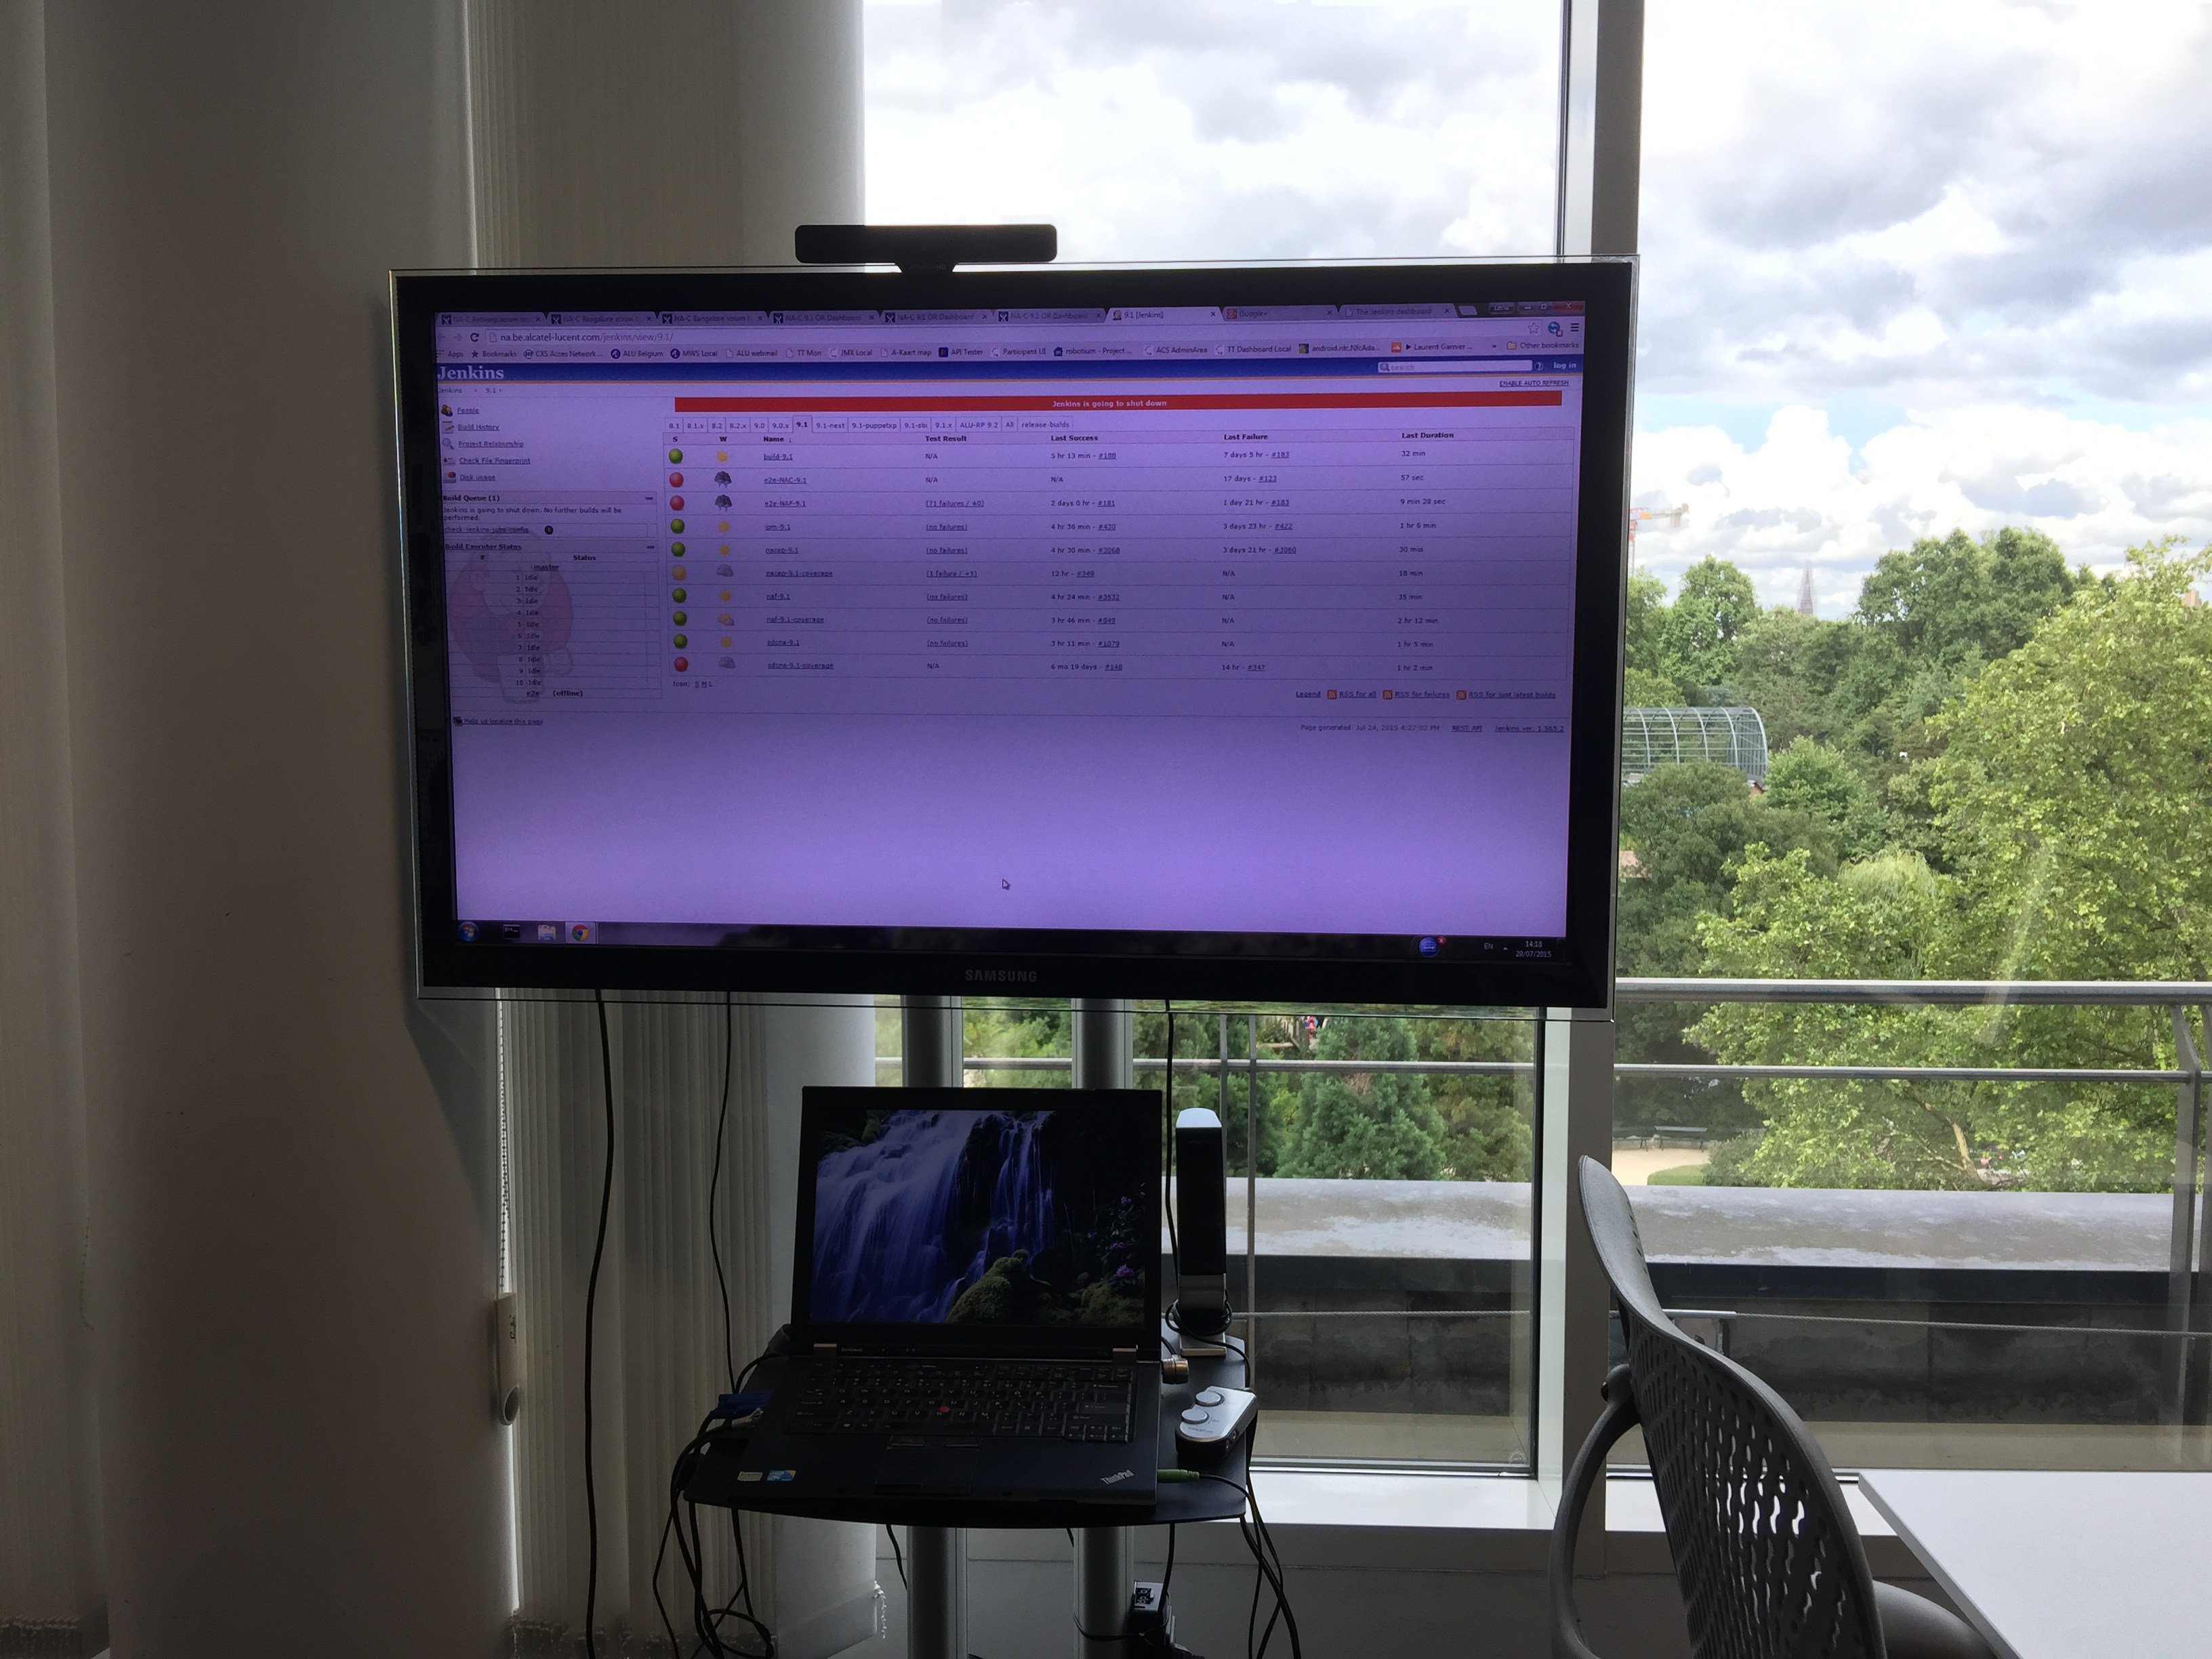
\includegraphics[width=90mm]{tvdashboardoriginal.jpg}
\caption{Het originele Jenkins dashboard weergegeven op de televisie op de afdeling van NA-C in Antwerpen.} 
\label{tv_1}
\end{figure}

\subsection{Stage-opdracht}
Mijn stage-opdracht bestond erin om Jenkins awareness te cre\"eren aan de hand van een dashboard dat een beter overzicht toont.
Als fouten meer in het oog springen, kunnen ze nog sneller verholpen worden en is er meer sprake van continuous integration. \todo{lame zin, maak beter!} Gedurende heel mijn stage werd ik enorm betrokken bij alles wat het team deed; zo deed ik dagelijks mee aan de stand-up meetings en werd ik meegevraagd in de sprint planning, sprint review en de retrospective, om zo een idee te krijgen hoe het er in een bedrijf aan toe gaat. Ook al kon ik niet meteen volgen waar ze het over hadden, het heeft me enorm veel bijgeleerd over hoe deze manier van werken het team sterker kan maken gezien iedereen (bijna) dagelijks updates krijgt over wie waarmee bezig is en de korte evaluatieperiodes ervoor zorgen dat er kort op de bal gespeeld kan worden.\\
Er werd voor gezorgd dat ik mijn eigen project kreeg, waarbij er dan ook tweewekelijkse sprints gepland werden, zodat ik een idee kreeg van hoe het eraan toe gaat. Er werd voor mij een JIRA-pagina aangemaakt, waarop ik mijn vooruitgang kon bijhouden door taken aan te maken die ik wou doen en problemen kon rapporteren. Een screenshot van mijn JIRA-dashboard is te zien in Figuur \ref{my_jira}.
Mijn eerste sprint bestond uit het maken van een literatuurstudie, op aanraden van Bart, om zo te zien waarop ik moet letten bij het maken van een (goed) dashboard en wat er verbeterd kan worden aan het originele Jenkins dashboard. Eens ik me een idee gevormd had van hoe ik wou dat het dashboard eruit zou zien, heb ik enkele voorstellen opgemaakt en een kleine enqu\^ete gemaakt binnen het team, om te kijken welke voorkeuren zij hadden. Hierop wordt dieper ingegaan in sectie \ref{sprint1}.\\
Vervolgens ben ik begonnen met het implementeren van het dashboard, dit was mijn tweede sprint. Het proces van hoe ik tot het resultaat ben gekomen, is te vinden in sectie \ref{sprint2}.\\
De derde en laatste sprint bestond uit het voorstellen van de eerste versie van het dashboard en hierover feedback krijgen, om het dashboard vervolgens te verbeteren. Tijdens de eindfase van deze sprint werd het dashboard in gebruik genomen op de Jenkins server van Alcatel-Lucent. Dit wordt besproken in sectie \ref{sprint3}.

\begin{figure}[ht!]
\centering
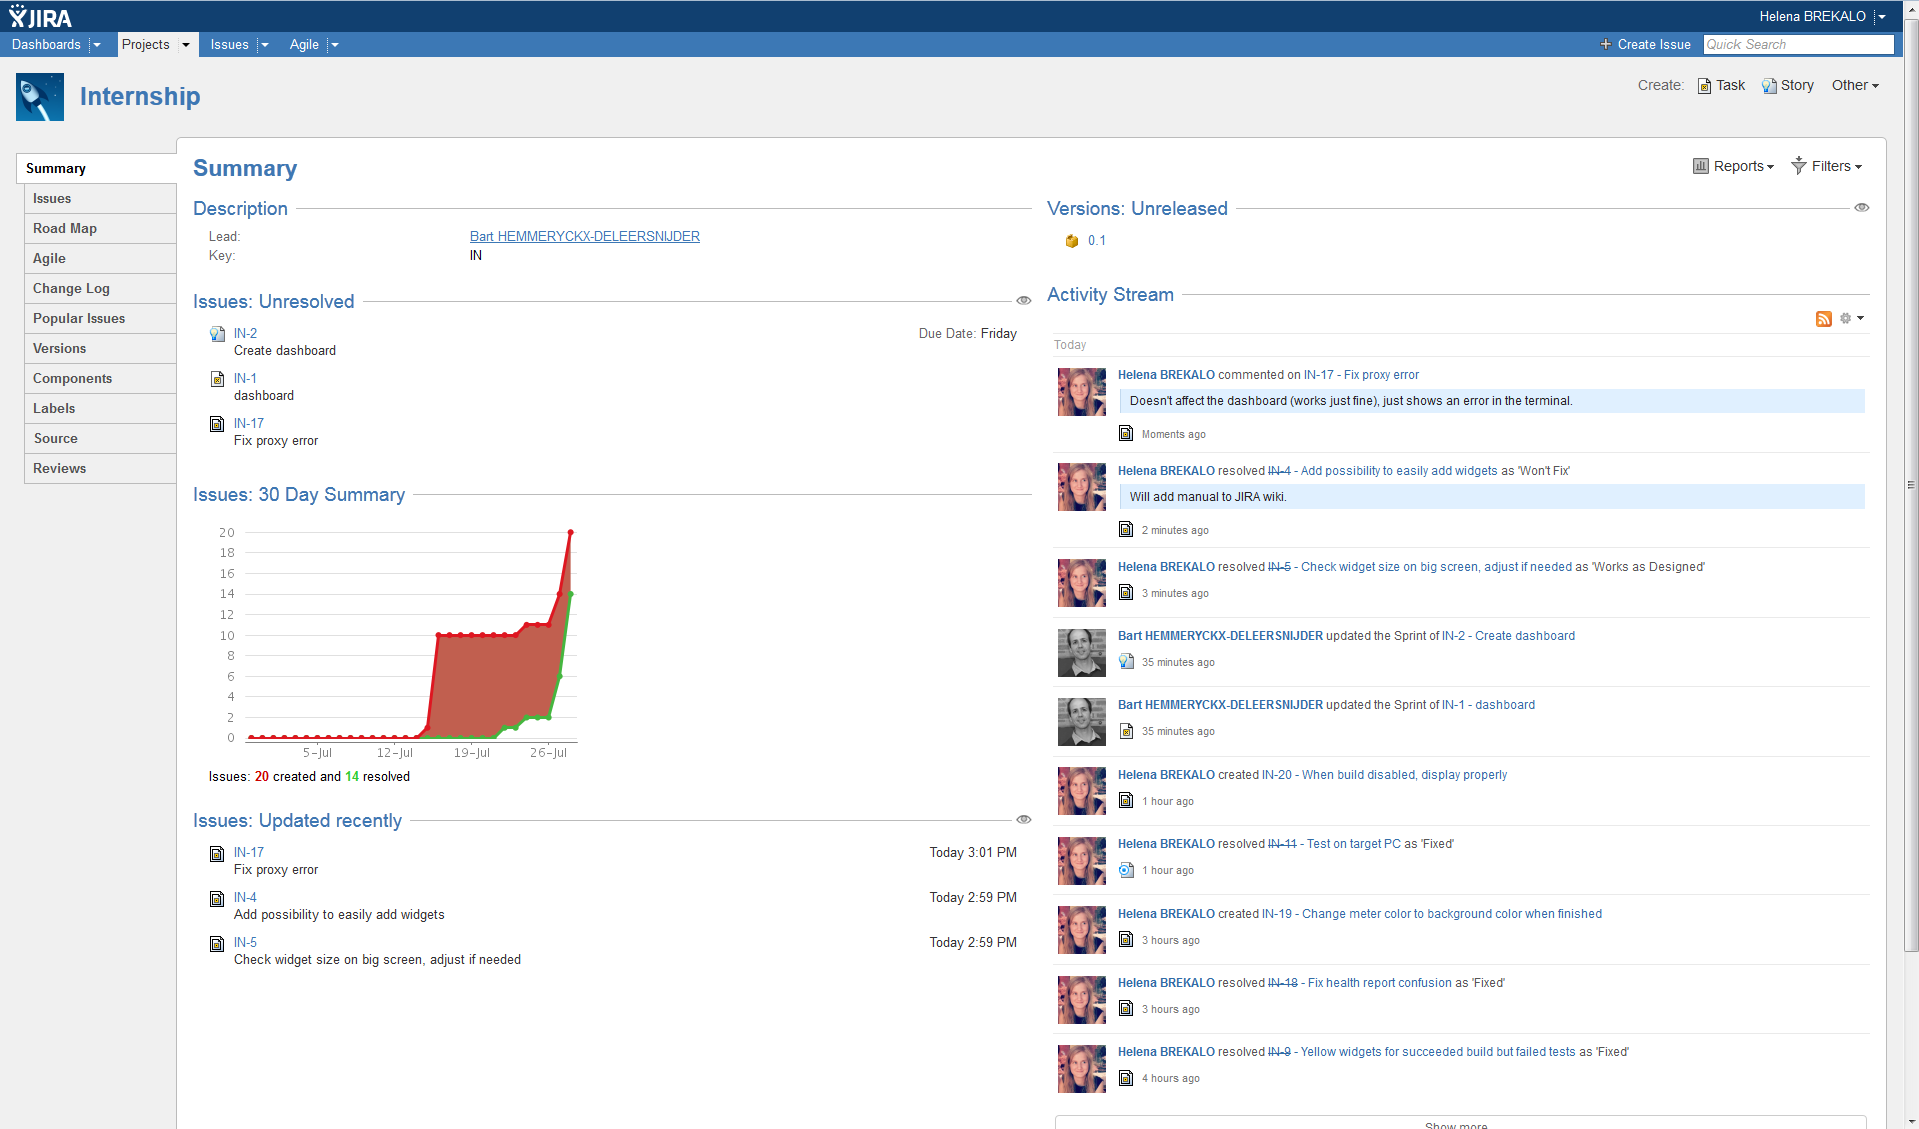
\includegraphics[width=90mm]{myJIRAscreenshot.png}
\caption{Het JIRA-dashboard voor mijn internship.} 
\label{my_jira}
\end{figure}

\subsubsection{Sprint 1: Onderzoek en literatuurstudie} 
\label{sprint1}
\paragraph{Literatuurstudie} Tijdens de eerste sprint heb ik onderzoek gevoerd naar hoe goede dashboards eruit zien en hoe je ze overzichtelijk kan houden. Hierrond heb ik een literatuurstudie gemaakt, die gevonden kan worden in de annex. \todo{anders verwoorden?} \todo{verwijzing} Uit deze literatuurstudie bleek inderdaad dat het voorziene Jenkins dashboard niet voldeed aan veel van de vereisten, aangezien je niet in \'e\'en oogopslag de belangrijkste info kan vergaren.\\
Naast de literatuurstudie heb ik ook gezocht naar tools om dashboards te maken, waarbij ik van een collega op de afdeling de aanbeveling kreeg om Dashing\footnote{http://dashing.io/} te gebruiken, waarbij hij ook een demo gaf. \todo{laatste deel zin weg?} Na het bekijken van nog enkele andere tools om dashboards te ontwikkelen, heb ik uiteindelijk voor Dashing gekozen, aangezien het enorm veel flexibiliteit biedt (je kan het dashboard helemaal inrichten zoals je wilt), \todo{deel tussen haakjes weg?} zodat ik het dashboard helemaal zou kunnen maken zoals ik het in gedachten had. \todo{anders verwoorden?}
\paragraph{Enqu\^ete}
Na het onderzoek en de literatuurstudie, heb ik een voorstel voor dashboardontwerpen gemaakt en deze voorgelegd aan de mensen bij NA-C. Ik liet hen hierbij een kleine enqu\^ete invullen waarbij ze konden kiezen voor verschillende designs en ook opmerkingen geven. Uit die opmerkingen zijn nog nuttige commentaren gekomen, bijvoorbeeld dat het tijdstip van de laatste build ook best getoond kan worden. De enqu\^ete en de resultatentabel zijn ook te vinden in de annex. \todo{referentie ernaar}
\subsubsection{Sprint 2: Ontwikkeling dashboard} 
\label{sprint2}
Op het einde van de eerste sprint heb ik met Bart een sprint review en retrospective gehouden, om te zien waar ik stond. We hebben deze meeting gecombineerd met de sprint planning, waarbij ik mocht aangeven hoe ik van plan was het dashboard uit te werken en met welke tools. Ik werd hierin heel vrij gelaten, zodat ik zelf kon ontdekken wat me lag en wat minder. \todo{beter verwoorden}
\paragraph{Gebruikte tools}
Dashing is een dashboard framework dat geschreven is in Sinatra (meer hierover in de volgende paragraaf), een open source software web applicatie geschreven in Ruby. De ontwikkeling gebeurde op Linux, waarbij ik gebruik maakte van Ubuntu 14.04. Op deze PC is dan een lokale Jenkins-omgeving opgezet, zodat ik het dashboard kon testen met mijn eigen projectjes. De code schrijven gebeurde in gedit zelf en debuggen werd gedaan via de terminal. \todo{nog zaken toevoegen?} \\
De "tegels" op het dashboard worden omschreven als "widgets" waarbij je verschillende soorten widgets kan hebben. Ik heb me toegespitst op een widget om informatie over Jenkins te tonen. Deze widget kan dan gebruikt worden voor verschillende builds, het is niet de bedoeling om voor elke build een nieuw widget te ontwikkelen (tenzij je andere informatie wilt tonen).
\paragraph{Gebruikte talen}
Het schrijven van het dashboard werd gedaan in verschillende talen, hieronder een opsomming welke taal wat voorzag \todo{anders zeggen?}.
\begin{description}
\item[HTML] HTML wordt gebruikt om te bepalen hoe de inhoud getoond wordt op de widget, dus welk deel als titel zal getoond worden en waar de elementen op de widget staan. De informatie die getoond wordt, wordt via Batman Bindings\footnote{http://batmanjs.org/} uit de JSON data van de Jenkins server geparset. \todo{klopt dit helemaal? Denk het wel.}
\item[(S)CSS] CSS wordt gebruikt om de tekst uit de HTML-file op te maken (grootte van de tekst, stijl, kleur,...), waarbij SCCS (Sassy CSS) ervoor zorgt dat je ook variabelen kan gebruiken, wat niet mogelijk is in standaard CSS. Op deze manier kan je dan (kleur)code hergebruiken via variabelen. \todo{beter zeggen}
\item[Javascript] Javascript werd gebruikt in de Batman Bindings, die ervoor zorgt dat de data die van de website geparset wordt, dynamisch gebruikt kan worden in de HTML-files (via data-bind).\todo{is dit te diep erop ingegaan?} Op zich is de Batman Bindings-library klaar om te gebruiken, maar om een tijdstip te parsen (dat werd weergegeven als Unix timestamp), heb ik nog enkele lijnen Javascript-code moeten toevoegen, alsook de moment.js-library.
\item[Coffeescript] Coffeescript is een taal die transcompileert naar Javascript. De .coffee-file voor het widget\todo{of de widget?} specifi\"eert hoe de data, die via de HTML-file opgevraagd wordt, weergegeven wordt. Deze file was van belang om bijvoorbeeld het juiste weerbericht te tonen. Het coffeescript parset\todo{juist vervoegd?} de data die via de Batman Bindings werd opgehaald en geeft aan hoe deze doorgegeven wordt aan de HTML-file. Zonder de .coffee-file zou er enkel \textit{plain text} te zien zijn op de widget.
\item[Ruby] Dashing maakt gebruik van Embedded Ruby om te bepalen welke tegels getoond worden op het dashboard en van plain Ruby om de data op te halen en te parsen vanuit de juiste plaats (nl. de Jenkins server) via de JSON-data die werd voortgebracht hierdoor. Ook wordt hier de link gelegd tussen de build jobs die getoond \emph{kunnen} (niet per s\'e zullen\footnote{Dat wordt bepaald door de Embedded Ruby file.}) worden op het dashboard.
\item[JQuery] JQuery wordt gebruikt in de Coffeescript file om CSS-gewijs klassen of ID's te gebruiken van elementen waarop je een bepaalde actie wil uitvoeren.
\item[JSON] JSON werd gebruikt om de data uit van de Jenkins server te parsen, zodat deze opgevraagd kon worden in de Ruby-file.
\end{description}
Omdat geen van deze talen me helemaal eigen was, heb ik enkele dagen genomen om de basics te leren via Codecademy\footnote{https://www.codecademy.com/}. Dit was voldoende om me op weg te zetten om zelf verder te experimenteren. \todo{dat laatste mss weglaten?}
De verschillende bestanden worden als volgt gebruikt:
\begin{itemize}
\item Een widget wordt opgesteld door middel van een .HTML-file, een .SCSS-file en een .coffee-file.
\item Een Embedded Ruby file geeft via HTML-blocks\todo{anders verwoorden?} aan welke build jobs getoond worden op het dashboard.
\item Een andere Embedded Ruby file doet de mapping van de JSON data op de variabelen in het dashboard en defini\"eert de namen van de build jobs die getoond kunnen worden.
\end{itemize}
\paragraph{Sprint Review} Op het einde van de tweede sprint werd mij gevraagd om de eerste versie van het dashboard te demonstreren voor het team in Antwerpen, Bangalor en Chennai. Ik kon een werkend dashboard tonen dat informatie toonde over de Jenkins build jobs die op mijn lokale server draaiden. Er waren geen opmerkingen of vragen.\todo{beetje droog, beter maken?}
\subsubsection{Sprint 3: Feedback en verbetering}
\label{sprint3}
Na de sprint review heb ik de Alcatel-Lucent Jenkins-server ge\"integreerd in het dashboard, wat nog anderhalve dag van debugging vroeg, gezien de Jenkins-server nu niet lokaal runde, maar op een andere server. Ook gebruikt men op Alcatel-Lucent een andere versie van Jenkins, waardoor bepaalde sleutelwoorden waarop geparset wordt anders heten.\\
Na de sprint retrospective van sprint 2 en de sprint planning van sprint 3 heb ik nog een enqu\^ete gedaan om positieve en negatieve puntjes te verzamelen waar men bij de voorstelling van het dashboard tijdens de demo misschien niet was opgekomen. De resultaten van deze enq\^ete zijn te vinden in de annex.\todo{verwijzing toevoegen}
\paragraph{Ingebruikname} \todo{over vertellen}
\subsection{Resultaat}
De eerste versie van het dashboard is te zien in Figuur \ref{dash_1}. Het dashboard in zijn huidige vorm is gemaakt om getoond te worden op een HD-televisie met 16:9 ratio. Het is de bedoeling dat er zes tegels naast elkaar kunnen staan en dat er drie rijen zijn, wat maakt dat de status van 18 build jobs gelijktijdig getoond kunnen worden. Dit bleek ruim voldoende voor het NA-C team, aangezien er altijd maar op enkele builds tegelijkertijd gefocust wordt.\todo{Indien er een definitieve (dwz veranderde) versie is, praat erover!}

\begin{figure}[ht!]
\centering
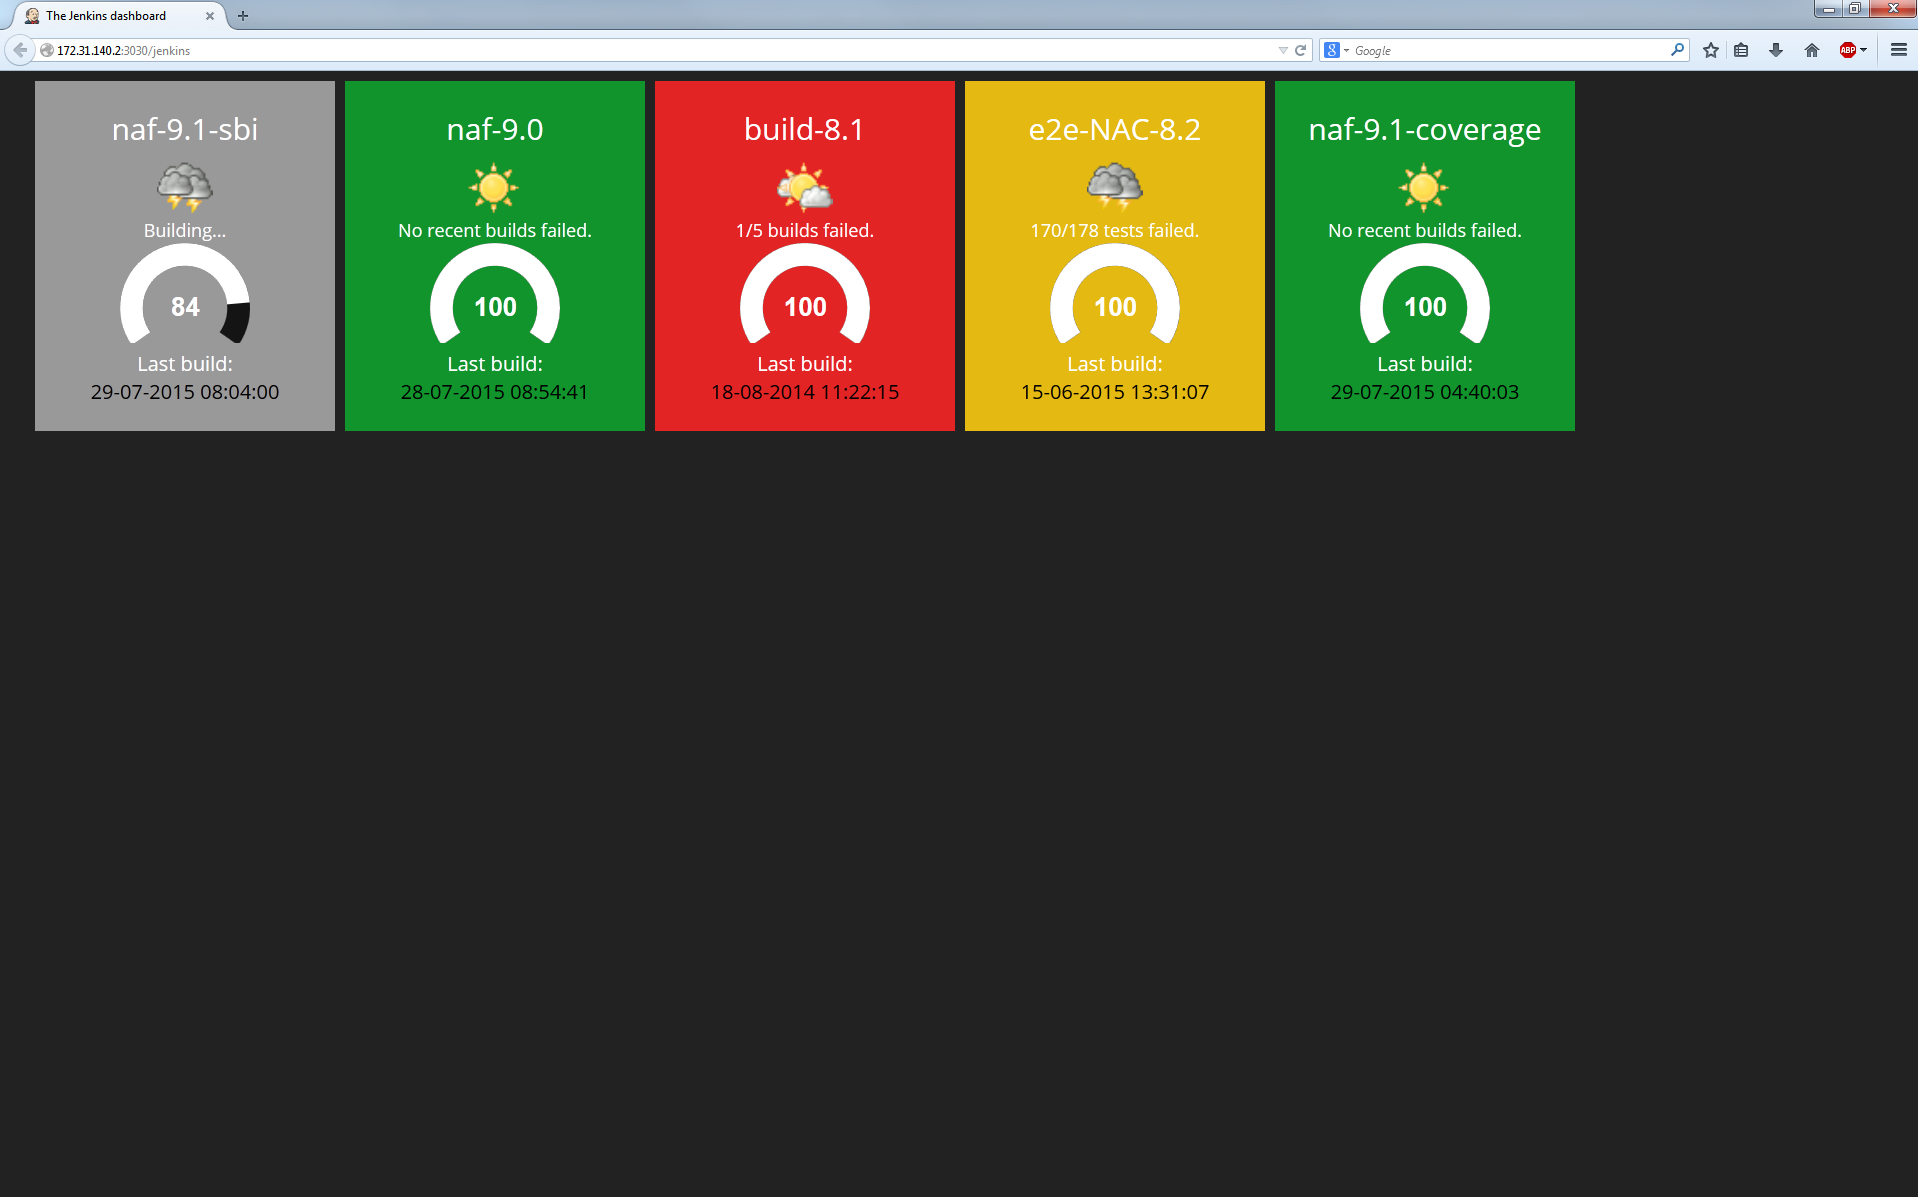
\includegraphics[width=90mm]{dashboard_screenshot1.png}
\caption{Gedetailleerd overzicht dashboard.} 
\label{dash_1}
\end{figure}

Figuur \ref{dash_2} toont de tegels in meer detail. De titel is de naam van de build waarover de tegel informatie verschaft. Het weerbericht toont de stabiliteit van de build, of, indien er testen gefaald zijn, de stabiliteit van de testen, de tekst eronder geeft aan hoe stabiel de builds/testen zijn, de meter geeft aan hoe ver de build is in zijn vooruitgang en de timestamp daaronder toont wanneer de laatste build uitgevoerd is.
Er zijn verschillende achtergrondkleuren gebruikt, die de status van de laatste build weergeven:
\begin{itemize}
\item Grijs: de build is nog bezig, het weerbericht toont de stabiliteit van de builds voor degene die nu bezig is.
\item Rood: de laatste build is gefaald.
\item Geel: \'e\'en of meerdere testen zijn gefaald.
\item Groen: alle builds zijn geslaagd en alle tests zijn geslaagd. 
\end{itemize}
Als er gekeken wordt naar het voorstel in de literatuurstudie, is de achtergrondkleur niet aanwezig (wel met een gekleurde bol), maar de rondvraagd op de afdeling toonde dat iedereen te vinden was voor de gekleurde achtergrond.

\begin{figure}[ht!]
\centering
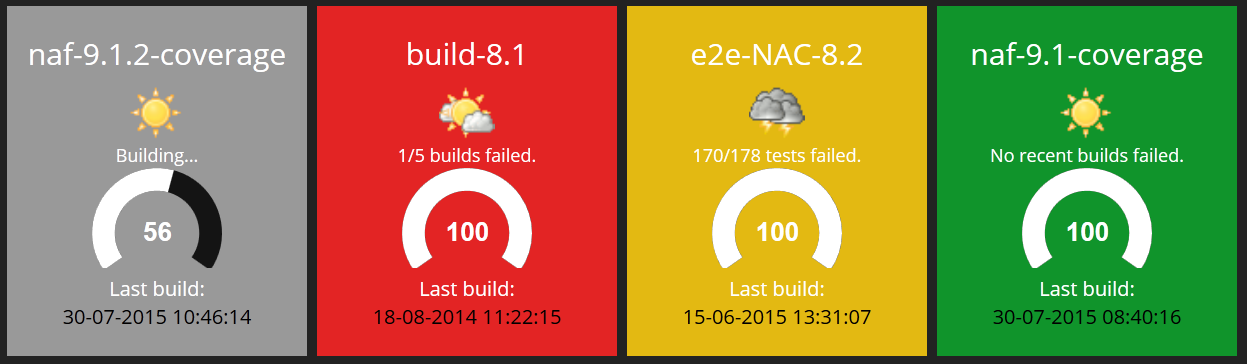
\includegraphics[width=90mm]{screenshot2.png}
\caption{Eerste versie van het dashboard.} 
\label{dash_2}
\end{figure}

\subsection{Initiatieven voor interns}
Alcatel-Lucent organiseerde deze zomer een initiatief om alle interns met elkaar in contact te brengen tijdens speciale info-events en meetings. Op deze manier konden interns van verschillende afdelingen met elkaar bespreken hoe de stage op hun afdeling verloopt en zo ervaringen met elkaar uitwisselen. Er zijn verschillende contactmomenten georganiseerd, meestal tijdens de middagpauze, waarbij er geluncht werd, er was een gesprek met bijeenkomsten: samen lunchen, infosessie over ALU Labs, gesprek met Joeri Veldeman, begonnen als doctor in de \textit{electrical engineering} bij Alcatel en nu hoofd van de afdeling van human resources. Zijn ongewone carri\`erepad werd ons uitgelegd en hij heeft informeel met ons gepraat over ons verdere studietrajecten.\\
Verder is er ook een infosessie geweest over ALU Labs, waarin enkele van de zaken aan bod kwamen waarin Alcatel-Lucent investeert en research bij uitvoert.\\
Dit alles maakte dat de stage niet alleen een verrijking van mijn kennis binnen de afdeling werd, maar ook daarbuiten, met nieuwe contacten tot gevolg.\todo{anders schrijven}

\section{Relatie stage en opleiding}
Het doel van de stage was om een dashboard te maken zodat de build status van de verschillende onderdelen van projecten overzichtelijk getoond konden worden. Binnen deze stage werd ik bovendien ook betrokken bij alle bijeenkomsten met het team, om zo te ervaren hoe het er in een werkomgeving aan toe gaat. Op deze manier heb ik extra facetten gezien die tijdens de opleiding aan bod zijn gekomen, die ik niet had gezien moest ik niet betrokken geweest zijn bij alles. Zo werkt men hier volgens de agile-methode scrum, met elke dag standup meetings en tweewekelijkse sprints. Dit is iets dat in de lessen van Software-Ontwerp kort aan bod was gekomen, waarvan ik tijdens de stage zag dat het echt zijn nut heeft. De korte sprints en regelmatige reviews zorgen ervoor dat problemen niet te lang kunnen blijven bestaan en door de continuous integration zijn mergefouten snel opgespoord en opgelost. Zelf kreeg ik ook eigen project, waardoor ik ook met sprints werkte en zo "kleine" doelen voor ogen had. Deze manier van werken is vergelijkbaar met die tijdens de P\&O-sessies tijdens de bachelorproef, waarbij we om de paar weken een bepaalde functionaliteit moesten kunnen demonstreren. Op de afdeling NA-C doet men ook regelmatig aan pair-programming, iets wat ook aangeraden was in de sessies van Software-Ontwerp. Aangezien ik aan een eigen project moest werken, heb ik dit niet zo vaak gedaan, maar als ik met vragen zat, kwamen collega's met plezier samen met mij zoeken.\\
Het dashboard dat ik moest maken moest niet een kant-en-klaar dashboard zijn dat ik gebruikte, waar ik dan zelf info aan toevoegde, maar een waarbij ik zelf moest nadenken over het design en de implementatie van de code om het dashboard te realiseren. Ik maakte gebruik van een bestaand framework, maar heb zelf nog heel veel van de code moeten schrijven. Dit heeft me er meer dan eens attent op gemaakt hoe belangrijk goede documentatie is, iets waar tijdens de lessen van Objectgericht Programmeren altijd op gehamerd is, aangezien het framework op zich nauwelijks/niet gedocumenteerd was en ik soms moeite had om te begrijpen wat een bepaalde functie deed. De documentatie op de websites van het framework en de plugins \todo{is dit het juiste woord?} was vaak ook erg kort door de bocht of onvolledig, dus ik heb vaak lang gezocht naar bepaalde zaken.\\
In de opleiding wordt er altijd gewerkt in kleine groepjes, meestal van twee mensen, maximaal in groepen van zes mensen. Op de afdeling NA-C werkt men in een team van ongeveer 10 mensen, wat het managaen van het team nog moeilijker maakt dan bij een groep van slechts enkele mensen. Toch is er getoond dat dit perfect mogelijk is indien je de juiste tools gebruikt (in dit geval Confluence en JIRA) en indien er genoeg gecommuniceerd wordt.\\
Tijdens de lessen van Informatica werktuigen zijn Ruby, Linux en LaTeX aan bod gekomen. Ruby bleek nuttig om de Embedded Ruby voor het dashboard te schrijven, waar de kennis van Linux ervoor zorgde dat ik iets vlotter mijn weg vond bij het installeren en werken met Linux, waar het dashboard in is ontwikkeld. LaTeX is gebruikt om de literatuurstudie te maken.\\
Doordat er in de bachelor informatica al een heel aantal programmeertalen gezien werden, was het aanleren van andere (opmaak)talen veel makkelijker. \\
Het schrijven van (wetenschappelijke) verslagen was een groot onderdeel tijdens Wetenschapscommunicatie en tijdens P\&O, wat me hielp bij het schrijven van de literatuurstudie en het stageverslag. \todo{te kort, moet nog tekst bijkomen}

\section{Krititsche reflectie competenties}
\begin{itemize}
\item Technische competenties die ik hoopte te verbeteren:
\begin{description}
\item[Bijleren over version control] Er wordt op de afdeling NA-C gewerkt met Git, waar ik ook tijdens mijn opleiding al mee in aanraking ben gekomen. Zelf heb ik niet echt gebruik gemaakt van Git, hoewel dit zeker nuttig geweest zou zijn bij het schrijven van mijn dashboard. Eens het dashboard klaar was, is het wel op Git gezet, maar dit had dus veel eerder moeten gebeuren.
\item[Leren werken met Jenkins] Op de afdeling NA-C werkt men met het continuous integration systeem Jenkins, dat builds automatisch runt nadat er een nieuwe versie van de software gecommit is. Tijdens de stage was het duidelijk hoe nuttig dit is: er werd op een gegeven moment een fout gemaakt, die ook nog eens onvoldoende getest bleek, maar men heeft deze heel snel ontdekt en binnen de 2 dagen kunnen oplossen. Moest er gewacht zijn met mergen tot vlak voor de release, was men waarschijnlijk veel meer problemen tegengekomen. Continuous integration is vooral handig in teams met meerdere mensen, het was dus van pas gekomen tijdens P\&O. \todo{dat laatste weglaten?}
\item[Mij inwerken in een reeds lopend project] Ik moest niet meewerken aan de code van het NA-C team zelf, maar heb mij wel moeten inwerken in de code van het dashboard. Zoals hierboven vermeld, was dit niet altijd makkelijk, maar het heeft er wel voor gezorgd dat ik enorm veel heb bijgeleerd, net omdat ik heel veel zelf moest uitzoeken. Eens de eerste versie van het dashboard klaar was, kende ik de code enorm goed, dus nieuwe veranderingen waren zeer snel gemaakt.
\end{description}
\item Persoonlijke competenties die ik hoopte te verbeteren:
\begin{description}
\item[Leren werken in grote teams] In het NA-C team in Antwerpen werken er een tiental mensen, in Bangalor en Chennai zijn er teams van gelijkaardige grootte.\todo{navragen!} Doordat er dagelijks een standup meetings was met de mensen van het team in Antwerpen, was iedereen goed op de hoogte van wie wat deed en doordat men met sprints van twee weken werkte, kwamen problemen en pijnpunten snel boven. Dit is iets dat ik zeker meeneem naar projecten in de toekomst toe, ik heb ervaren hoe al deze zaken kunnen helpen in het beter doen verlopen van een project.
\item[Plannen op lange termijn] Aan het begin van mijn stage werd me meteen gezegd dat ik redelijk vrij gelaten ging worden in mijn planning, maar er werd wel gevraagd om er een op te stellen, zodat ik ook in sprints kon werken. Ik heb zelf voorstellen mogen doen en aan mijn eigen tempo (maar toch binnen de termijnen van de sprints) kunnen werken. Als er grote dingen te doen stonden, plande ik daar altijd genoeg tijd voor in, zodat ik uiteindelijk "te vroeg" klaar was en aan verbeteringen kon werken. Dit is een van de competenties die ik zowel in het tweede semester van mijn laatste bachelorjaar heb aangescherpt, als nu op de stage.  
\end{description}
\end{itemize}

\section{Conclusie}

\section{Annex}

\end{document}